\documentclass[a4paper,oneside,10pt]{report}

\usepackage[USenglish]{babel} 
\usepackage[T1]{fontenc}
\usepackage[ansinew]{inputenc}

\usepackage{lmodern} %Type1-font for non-english texts and characters


%% Packages for Graphics & Figures %%%%%%%%%%%%%%%%%%%%%%%%%%
\usepackage{graphicx} %%For loading graphic files
%\usepackage{subfig} %%Subfigures inside a figure
%\usepackage{pst-all} %%PSTricks - not useable with pdfLaTeX

%% Please note:
%% Images can be included using \includegraphics{Dateiname}
%% resp. using the dialog in the Insert menu.
%% 
%% The mode "LaTeX => PDF" allows the following formats:
%%   .jpg  .png  .pdf  .mps
%% 

%% Math Packages %%%%%%%%%%%%%%%%%%%%%%%%%%%%%%%%%%%%%%%%%%%%
\usepackage{amsmath}
\usepackage{amsthm}
\usepackage{amsfonts}

%% Line Spacing %%%%%%%%%%%%%%%%%%%%%%%%%%%%%%%%%%%%%%%%%%%%%
%\usepackage{setspace}
%\singlespacing        %% 1-spacing (default)
%\onehalfspacing       %% 1,5-spacing
%\doublespacing        %% 2-spacing


%% Other Packages %%%%%%%%%%%%%%%%%%%%%%%%%%%%%%%%%%%%%%%%%%%
%\usepackage{a4wide} %%Smaller margins = more text per page.
\usepackage{fancyhdr} %%Fancy headings
%\usepackage{longtable} %%For tables, that exceed one page

\usepackage{color}

\newcommand{\cs}{\texttt{C\#}}
\newcommand{\textcode}[1]{\vspace{0.3em} \newline  \hspace*{2em} \texttt{\footnotesize{#1}} \newline \vspace{0.3em}}
\newcommand{\codeindent}{\hspace*{4em}}
\newcommand{\todo}[1]{{\Large \color{red}{\# #1\ \#}}\newline}

% Remove chapter numbering
\renewcommand*\thesection{\arabic{section}}
\renewcommand*\thesubsection{\arabic{section}.\arabic{subsection}}
\renewcommand*\thesubsubsection{\arabic{section}.\arabic{subsection}.\arabic{subsubsection}}
\setcounter{secnumdepth}{4}



%%%%%%%%%%%%%%%%%%%%%%%%%%%%%%%%%%%%%%%%%%%%%%%%%%%%%%%%%%%%%
%% DOCUMENT
%%%%%%%%%%%%%%%%%%%%%%%%%%%%%%%%%%%%%%%%%%%%%%%%%%%%%%%%%%%%%
\begin{document}

\pagestyle{empty} %No headings for the first pages.

%% Title Page %%%%%%%%%%%%%%%%%%%%%%%%%%%%%%%%%%%%%%%%%%%%%%%

\title{Transaction Management System}
\author{Michael J. Hunter}
%\date{} %%If commented, the current date is used.
\maketitle

%% TOC %%%%%%%%%%%%%%%%%%%%%%%%%%%%%%%%%%%%%%%
\tableofcontents %Table of contents
\cleardoublepage %The first chapter should start on an odd page.

\pagestyle{plain} %Now display headings: headings / fancy / ...

This document outlines the design of the Transaction Management system, which is a software application suite encompassing the CCTM (Credit Card Transaction Manager) and the RTCC (Real-Time Credit Cards). This is aimed at software maintenance engineers to get an understanding of the underlying architecture and design of the software.

\section{System Overview}

The purpose of the Transaction Management System is to authorize credit card transactions received from directly or indirectly from Single Space Parking Meters. Authorization can be performed using a variety of different authorization platforms, such as Montra or CreditCall. The two main systems, CCTM and RTCC, differ in the way that they acquire transactions - the CCTM acquires transactions from a database in a non-real-time manner, and the RTCC acquires transactions directly from the parking meter.
The system is implemented primarily in the managed .NET environment of \cs{} using Visual Studio, since it is primarily a high-level application suite involving logic and user interaction. Required performance is low, at perhaps a few transactions per second.

An overview of the architecture of the entire software suite is shown in Figure \ref{fig:SuiteOverview}. Since the CCTM and RTCC perform similar operations, they are treated only as logic and GUI extensions of what is called the Transaction Management System.

\begin{figure}
	\centering
		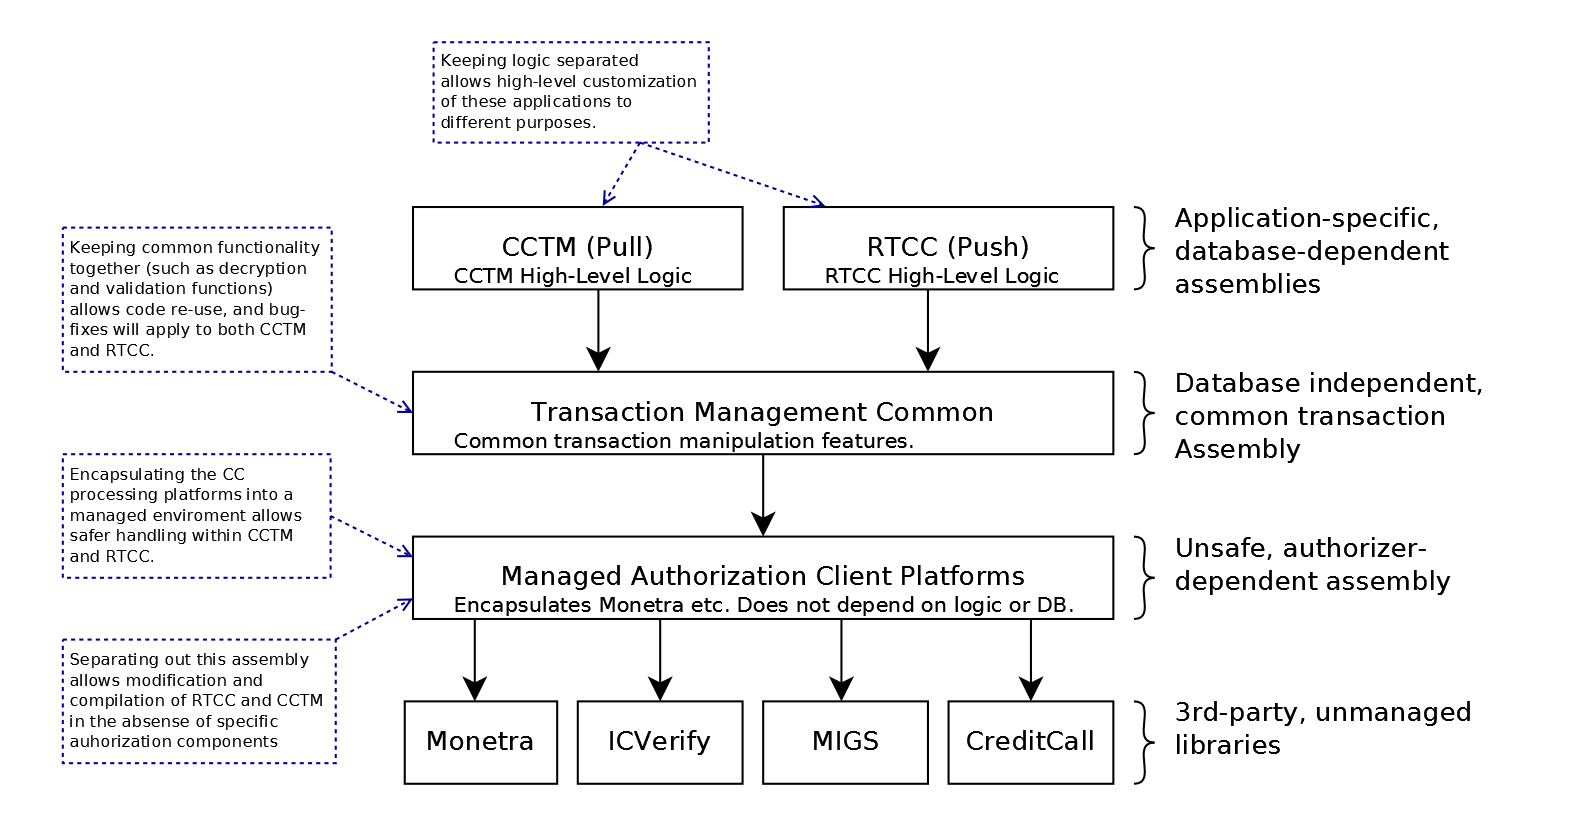
\includegraphics[width=1.0\textwidth]{RTCC_CCTM_Layers.png}
	\caption{Transaction Management Suite overview}
	\label{fig:SuiteOverview}
\end{figure}

\subsection*{CCTM}
The CCTM is an application which retrieves unprocessed credit card transactions from a database and processes them using one of a number of authorization platforms. It is responsible for the high-level logic and behavior of the delayed (asynchronous) authorization, using common functionality provided by the Transaction Management Common library and its dependencies (see below).
\subsection*{RTCC}
The RTCC is an application which synchronously processes credit card transactions provided in real-time from a parking meter. Similar to the CCTM, it is responsible for the high-level logic and behavior of the real-time authorization.

\subsection*{Transaction Management Common}
This is a library which provides high-level functionality specific to the Transaction Management System (to process credit card transactions) but common to both the RTCC and CCTM. Although represented in Figure 1 as a single entity common to both the CCTM and RTCC, it may be deployed separately for the two applications. This library is independent of third-party modules, and allows software maintenance without the lengthy process of setting up the development environment with third-party modules.
\subsection*{Authorization Client Platforms}
This is a library which provides functionality for authorizing credit cards using a predefined suite of authorization processors/platforms. As well as providing functionality common to credit card operations, this library provides a standardized, managed abstraction of the various authorization platforms.
\subsection*{Cryptographic Platforms}
This is a library which exposes objects for handling the types of encryption used by the Transaction Management System for securing credit card information.

\section{CCTM}
\subsection{Primary CCTM Dimensions}
As shown in Figure \ref{fig:CCTMDimensions}, the primary dimensions of the CCTM are the GUI, runtime configuration and the CCTM Mediator. The mediator, as described in Section \ref{sec:CctmMediator}, provides the high-level system logic, and answers the question ``what happens?''. The term ``runtime configuration'' is used here to refer to the entities which link the CCTM from its basic componenents. Due to the nature of a Visual Studio Windows Forms application, the runtime configuration is integrated into the GUI: when the main form is launched, it constructs and initializes the CCTM.

\begin{figure}
	\centering
		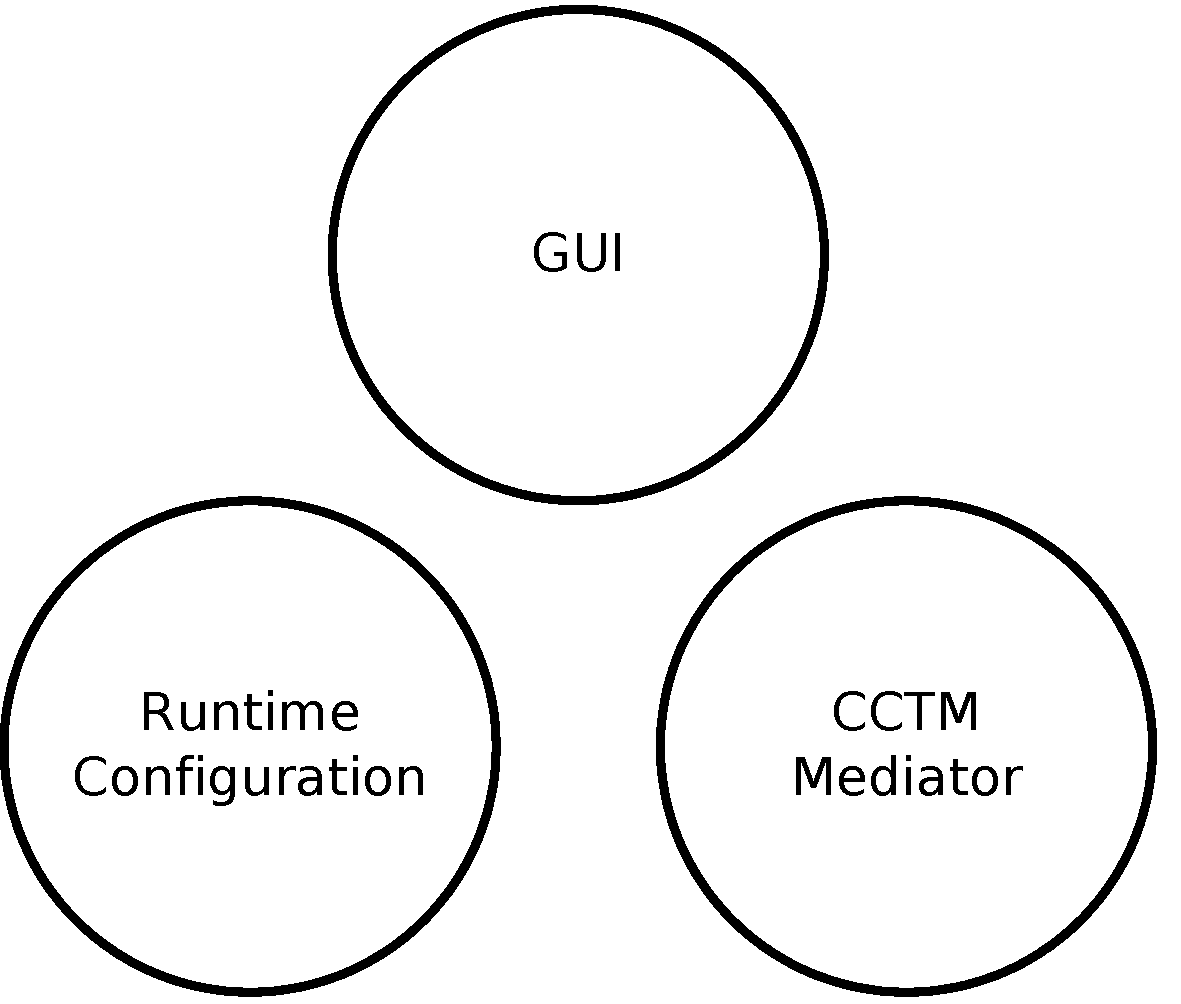
\includegraphics[width=0.4\textwidth]{CCTM_Dimensions.pdf}
	\caption{CCTM Dimensions}
	\label{fig:CCTMDimensions}
\end{figure}

Each of these components is interlinked, and can individually be thought of as the ``head'' of the application, depending on what perspective you take. The GUI is the head because it is the source of initial control. The mediator is the head because it controls what the CCTM does at a high level, and ties all the pieces together \emph{logically} - the logic behind what happens. The runtime configuration is the head because it manages the runtime linking of all the pieces.

\subsection{GUI}



\subsection{CCTM Mediator}\label{sec:CctmMediator}
An overview of the function of the CCTM is shown in Figure \ref{fig:CCTMFlow}. Unprocessed transaction records are fetched from the database, and the mediator logic processes them by parsing the record data, decrypting if necessary, authorizing, and recording the result to the database. The CCTM Mediator is built on abstractions to handle all of those functions, and is named such because it provides the mediation between all of those components.

\begin{figure}
	\centering
		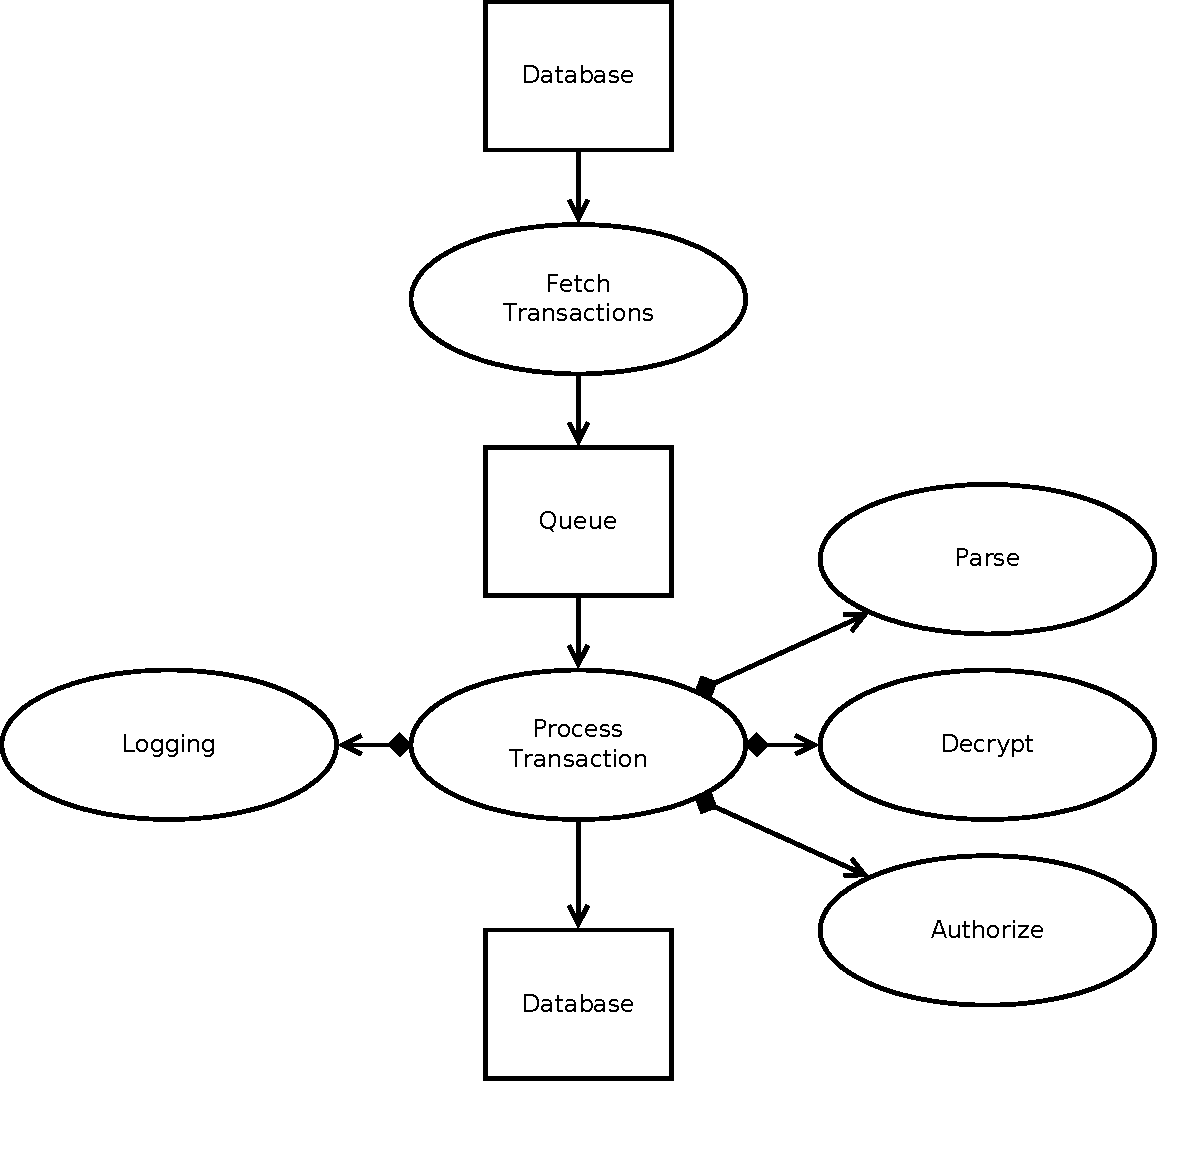
\includegraphics[width=0.8\textwidth]{CCTM_Flow.pdf}
	\caption{CCTM Information and Processing Flow}
	\label{fig:CCTMFlow}
\end{figure}

\section{Common}
\subsection{Server Controller}
One of the primary functions of the Transaction Management System is to orchestrate the interaction of networked client and server objects. Such servers include the SQL server and credit card processors such as Monetra. T utilize these servers, the Transaction Management System needs to maintain an active connection to the server. The logic behind the server management can be complicated, and is essentially the same each server and for each operation on the server. 

Consider Figure \ref{fig:SOL} as an example of the type of process flow involved in a server operation. In addition to flow control logic, the server controller needs to manage the multi-threaded aspect of a server: generally multiple clients can perform operations at once, but in the case of a failure only one thread can attempt to restart (or reconnect) the server, and during that time other threads must wait until the server is restarted to perform operations. 

\begin{figure}
	\centering
		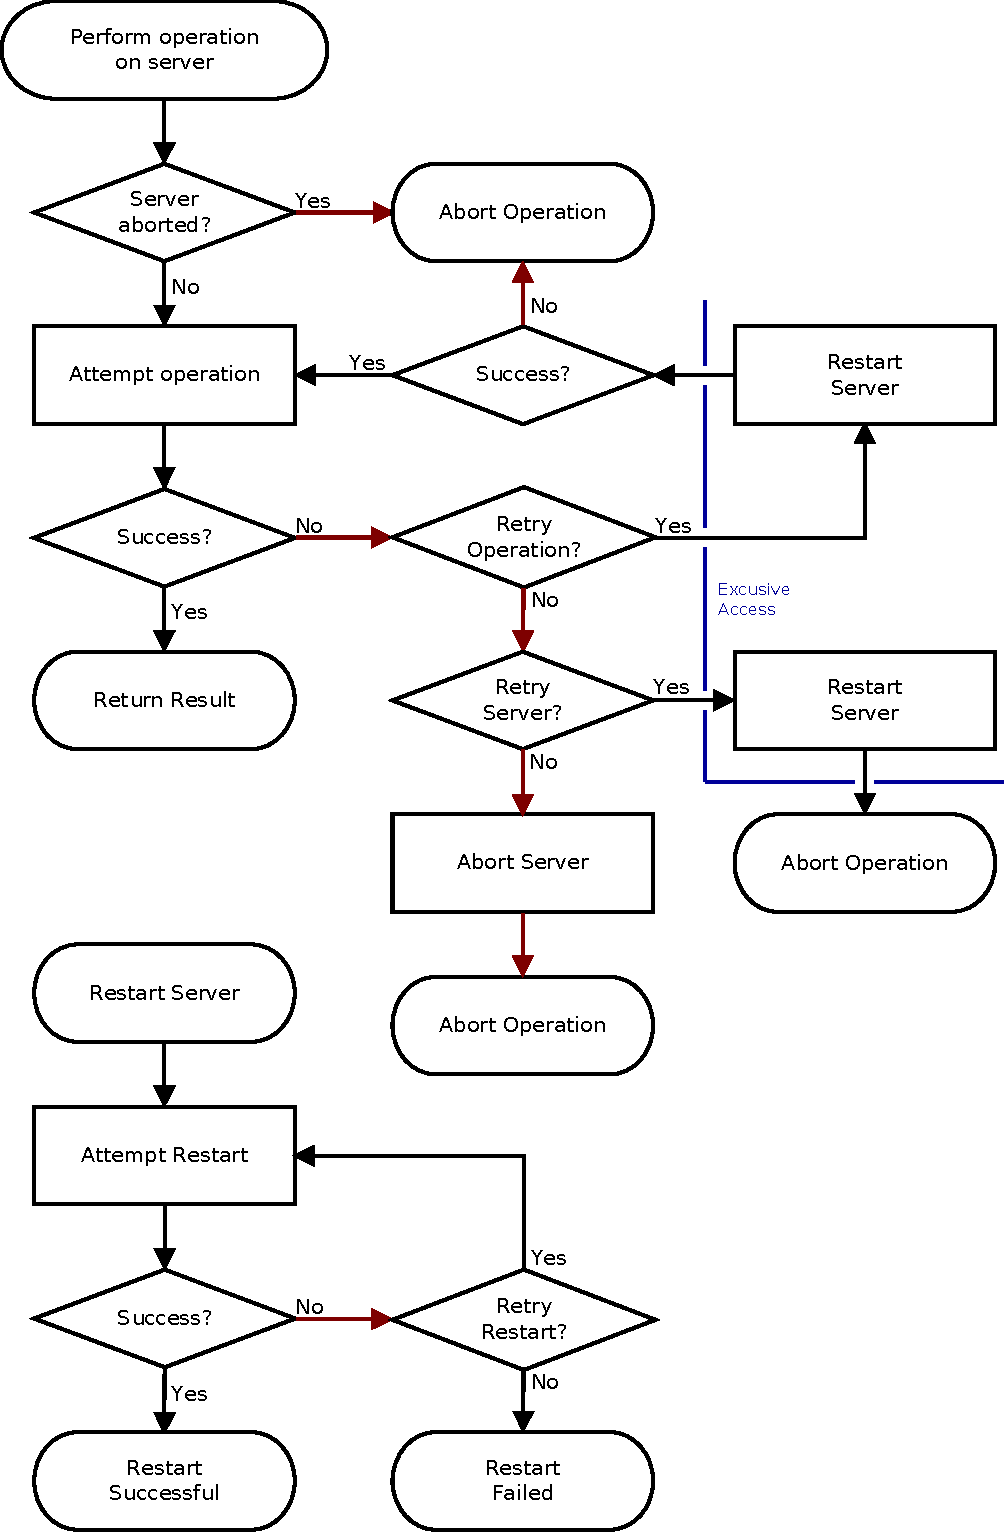
\includegraphics[width=1.0\textwidth]{ServerOperationLogic.pdf}
	\caption{A generic flowchart to perform an operation on a remote server}
	\label{fig:SOL}
\end{figure}

A server controller provides a layer through which a ``server'' may be accessed. In this case, the term ``server'' is used to describe any object which provides functionality, and more usefully in this case, objects that exposes this functionality by accessing a remote, networked server object. A ``server'' in this case is most likely to fail because of a connectivity (state) proglem, which can most often be corrected by resetting the state of the representative object (such as resetting the connection to the server). The primary function of a server controller is to manage the state of the server. Figure \ref{fig:ServerControllerState} illustrates the states a Server Controller manages for its server.

\begin{figure}
	\centering
		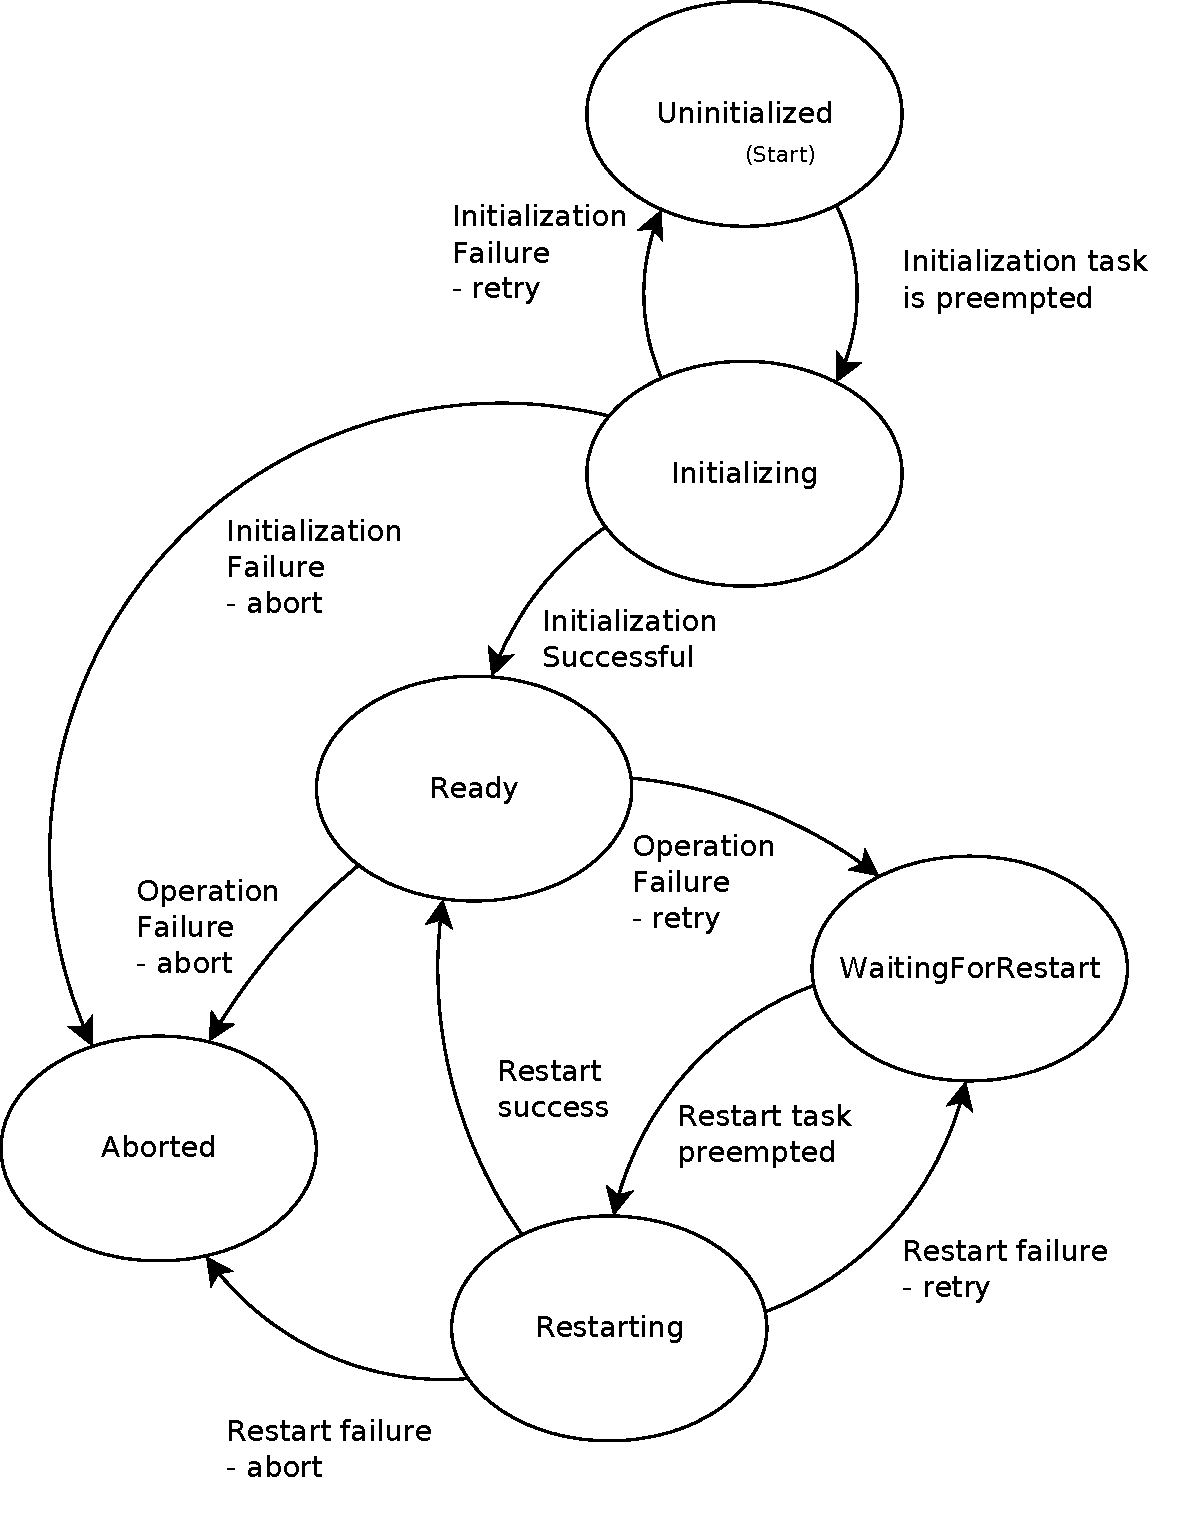
\includegraphics[width=0.9\textwidth]{ServerControllerState.pdf}
	\caption{Server states managed by the Server Controller}
	\label{fig:ServerControllerState}
\end{figure}

Figure \ref{fig:ServerControllerCD} illustrates the possible use of a Server Controller. A Server, such as the Monetra Client (because it directly represents the Monetra Server), performs operations by exposing an interface. These operations are performed by causing the Server Controller to perform them on the server. This notation is not completely transparent since the Server Controller is unable to implement the server's interface, so generally a controller adapter will we created which represents the controller as if it were the server itself by implementing the server's primary interface. To make the generation of server controller adapters easier, a \texttt{ControllerWrapper} template class is a base class from which specific adapters can be established. 

\begin{figure}
	\centering
		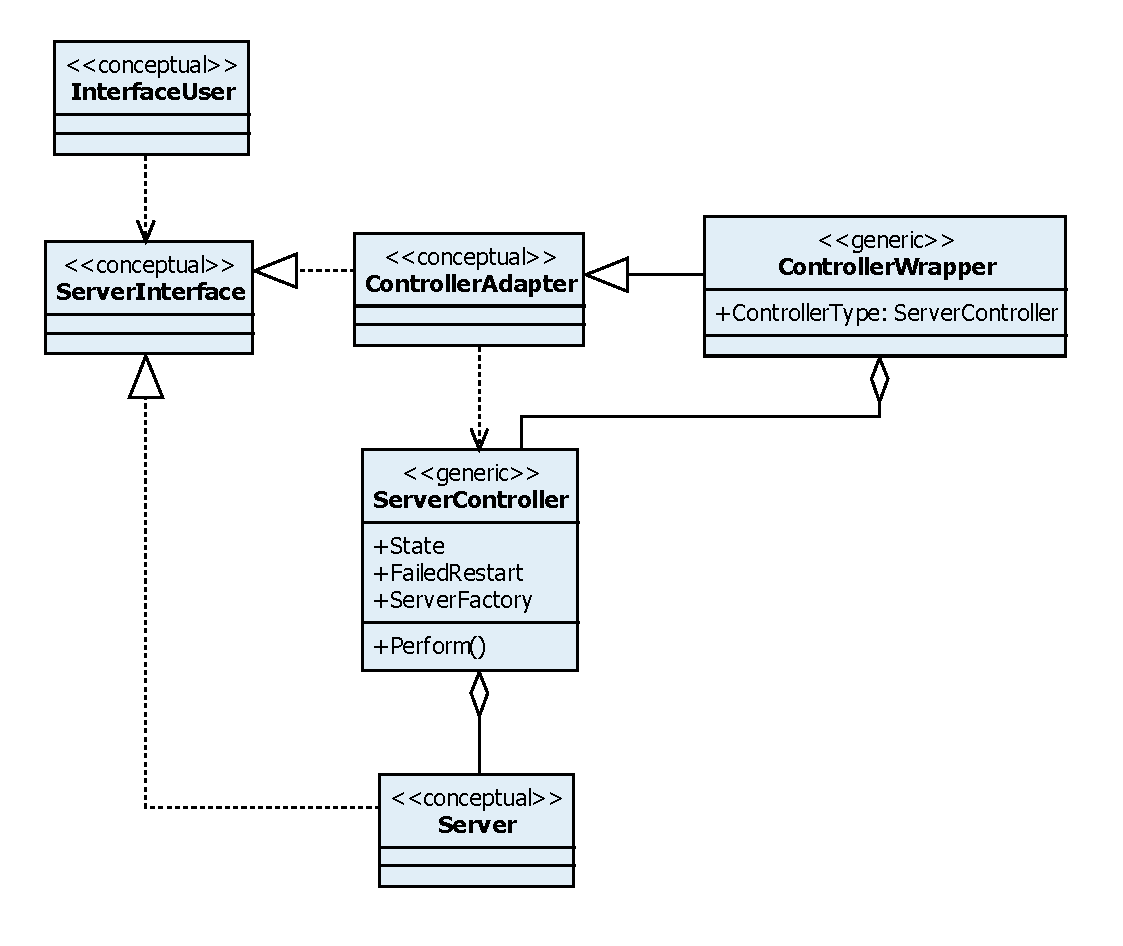
\includegraphics[width=0.9\textwidth]{ServerControllerClassDiagram.pdf}
	\caption{General use of a Server Controller}
	\label{fig:ServerControllerCD}
\end{figure}

A \texttt{ServerController} is conceptually a meta-class for a server, redefining traditional class behavior such as operation calls or instantiation and destruction. Since there is no language support in \cs{} for overriding such class behavior, this has been done manually through the use of a generic \texttt{ServerController} class, type-parametrized methods, and lambda expressions. Performing an opereration like \textcode{MyData = MyDatabase.GetData();} is now be done like \textcode{MyDatabaseController.Perform(\newline \codeindent (database) => \{ MyData = database.GetData(); \} );} or \textcode{MyData = MyDatabaseController.Get<MyDataType>( \newline \codeindent(database) => database.GetData() );} allowing the controller to manage the exact behavior of the operation. This can be thought of as asking the controller to perform a specific operation on the server, and the controller determines when to execute it and how many times to execute it etc.

%%%%%%%%%%%%%%%%%%%%%%%%%%%%%%%%%%%%%%%%%%%%%%%%%%%%%%%%%%%%%



%%%%%%%%%%%%%%%%%%%%%%%%%%%%%%%%%%%%%%%%%%%%%%%%%%%%%%%%%%%%%
%% BIBLIOGRAPHY AND OTHER LISTS
%%%%%%%%%%%%%%%%%%%%%%%%%%%%%%%%%%%%%%%%%%%%%%%%%%%%%%%%%%%%%
\addtocontents{toc}{\protect\vspace*{\baselineskip}}

%%%%%%%%%%%%%%%%%%%%%%%%%%%%%%%%%%%%%%%%%%%%%%%%%%%%%%%%%%%%%
%% APPENDICES
%%%%%%%%%%%%%%%%%%%%%%%%%%%%%%%%%%%%%%%%%%%%%%%%%%%%%%%%%%%%%
\appendix

\end{document}

